\graphicspath{{Figures/}}
%\pagenumbering{arabic}
\chapter{Commande Optimale} \label{chap:optimal control}
\section{Préliminaires et définitions fondamentales}
\subsection{Conditions suffisantes et nécessaires pour la stabilité des systèmes linéaires stationnaires}\label{subsec-chap2:CNS stabilité syslin}
Considérons le système :
\begin{equation}\label{eq-chap2:syslin}
	\stateDot = \matriceA\state.
\end{equation}
L'origine du système~\eqref{eq-chap2:syslin} est asymptotiquement (dans ce cas, exponentiellement) stable si et seulement si, pour toute matrice $\mathbf{Q}$ symmétrique définie positive, il existe une matrice $\mathbf{P}$ symmétrique définie positive solution de l'Équation de Lyapunov~\eqref{eq-chap2:LyapEq} : 
\begin{equation}\label{eq-chap2:LyapEq}
 	\matriceP\matriceA + \matriceA^T\matriceP = -\matriceQ
\end{equation}
\paragraph{Preuve :} $(\Rightarrow)$ On suppose que l'équation~\eqref{eq-chap2:LyapEq} est vraie.  On définit la fonction $V=\state^T\matriceP\state$ définie positive. La dérivation par rapport au temps donne : 
\begin{align}
	\begin{split}
		\dot{V} =& \stateDot^T\matriceP\state + \state^T\matriceP\stateDot \\
		\eqref{eq-chap2:syslin} \Rightarrow\dot{V} =& \state^T\matriceA^T\matriceP\state + \state^T\matriceP\matriceA\state \\
		\eqref{eq-chap2:LyapEq} \Rightarrow\dot{V} =& -\state^T\matriceQ\state 
	\end{split}
\end{align}
Par la vertue du deuxième théorème de Lyapunov, l'origine du système~\eqref{eq-chap2:syslin} est asymptotiquement stable. 

$(\Leftarrow)$ {\color{red} HERE}
\subsection{Commandabilité et obervabilité}
Soit le système linéaire suivant : 
\begin{align}\label{eq-chap2:syslin_commande}
	\begin{split}
		\stateDot &= \matriceA\state+\matriceB\command, \ \state\inR^n, \ \command\inR^m,\\
		\out &= \matriceC\state, \ \out\inR^p
	\end{split}.
\end{align}
\subsubsection{Commandabilité} La paire $\left(\matriceA,\matriceB\right)$ dy système~\eqref{eq-chap2:syslin_commande} est commandable si pour chaque état initial $\state(t_0)$, il existe $\command_{\left[t_0,t_1\right]}$ tel que $\state(t_0)$ est transféré vers $\state(t_1)$ en temps fini. 
Une condition suffisante pour vérifier la commandabilité est de vérifier si ${\rm{rang}}\left(\left[\matriceB \ \matriceA\matriceB \ \matriceA^2\matriceB \ \ldots \ \matriceA^{n-1}\matriceB\right]\right)=n$.

\subsubsection{Observabilité} La paire $\left(\matriceA,\matriceC\right)$ est observable si les trajectoires de l'état du système $\state(t)$ peuvent être estimées à partir de la sortie $\out(t)$ et la commande $\command(t)$. Une condition suffisante pour vérifier l'observabilité est de vérifier si ${\rm{rang}}\left(\begin{bmatrix}
	\matriceC \\ \matriceC\matriceA \\ \matriceC\matriceA^2 \\ \vdots\\ \matriceC\matriceA^{n-1}
\end{bmatrix} \right)=n$.
\section{Motivation : pourquoi la commande optimale ?}

Soit le système~\eqref{eq-chap2:syslin_commande}. Si la paire $(\matriceA,\matriceB)$ est commandable, il est possible de choisir une commande par retour d'état $\command = -\matriceK\state$ pour stabiliser l'origine en boucle fermée. La matrice de gains $\matriceK$ peut être choisie pour placer arbitrairement les pôles de la matrice $\matriceA -\matriceB\matriceK$ à gauche de l'axe imaginaire. En effet, à fur et à mesure que l'on s'éloigne à gauche l'axe imaginaire $(\Re(\lambda_i)<<0)$, la réponse du système en boucle fermée devient de plus en plus rapide. Cela se concrétise par par une convergence rapide de $\state$ vers l'origine. Malheuresement, cette dynamique rapide requiert typiquement de grandes amplitudes de a commande $\command$. Ces amplitudes peuvent  excéder les limites maximales admissibles, voire même exciter des modes non modélisés. 

Cette problématique nous mène à se demander si on peut trouver une matrice des gains $\matriceK$ qui assure  :
\begin{itemize}
	\item La stabilité du système
	\item La minimisation d'un critère d'optimalité $J$
\end{itemize}
Un tel gain $\matriceK$ est dit \emph{optimal}. 

\section{Types de critères}
Plusiers critères  peuvent être considérés :
\begin{itemize}
	\item Somme des valeurs absolues $J(\state) = \sum ||\state(t)||_1$
	\item Somme des normes Eclidéenne $J(\state) = \sum ||\state(t)||_2$
	\item Somme des carrés $J(\state) = \sum ||\state(t)||_2^2$
	\item Somme des normes infinie $J(\state) = \sum ||\state(t)||_{\max}$
\end{itemize}
Parmis tous ces critères, celui de la somme des carrés possède des propriétés mathématiques intéréssantes et qui facilitent sa manipulation, notamment la dérivabilité de $J(\state)$ et la continuité de sa dérivée. On peut aussi inclure l'énergie dépensée en termes de commande (effort) $J(\state) = \sum q||\state(t)||_2^2 + r||\command(t)||_2^2$. 

De manière générale, le problème de la commande optimale revient à résoudre :
\begin{align}\label{eq-chap2:gen optimal problem}
	\begin{split}
		\underset{\command}{\min}~&{\cal J}(\state,\command,\tau) \\
		{\rm s.c}~&\stateDot = f(\state,\command)
	\end{split},
\end{align}
où la fonction-coût ${\cal J}=(\state,\command,\tau) = \int_0^t{\cal L}(\state,\command,\tau)d\tau$ avec ${\cal L}(\state,\command,\tau)$ représente une certaine norme.

\section{Commande linéaire quadratique (LQR)}
Dans le cas d'une commande linéaire quadratique (anglais : Linear Quadratic Regulator (LQR)), ${\cal L}(\state,\command)$\footnote{La dépendance par rapport au temps est homise car le système que l'on traite est linéaire stationnaire~\eqref{eq-chap2:syslin_commande}} s'exprime comme : 
\begin{equation}\label{eq-chap2:form LQR}
	{\cal L}(\state,\command) = \fracOneTwo\left(\state^T\matriceQ\state + \command^T\matriceR\command\right).
\end{equation}
La forme quadratique de ${\cal L}$~\eqref{eq-chap2:form LQR} en fonctions de $\state$ et de $\command$ donne le nom à la commande, où $\matriceR\inR^{m\times m}$ (matrice \textbf{symmétrique définie positive}) et $\matriceQ\inR^{n\times n}$ (matrice \textbf{symmétrique semi-définie positive}) sont des matrices de poids de pénalisation de $\command$ et $\state$, respectivement. En effet, ${\cal L}$ représente un compromis entre l'effort de commande et la rapidité de convergence.

Dans le problème LQR, le problème d'optimisation~\eqref{eq-chap2:gen optimal problem} s'écrit comme : 
 \begin{align}\label{eq-chap2:LQR optimal problem}
 	\begin{split}
 		\underset{\command}{\min}~&\fracOneTwo\int_0^t\left(\state^T\matriceQ\state + \command^T\matriceR\command \right)d\tau\\
 		{\rm s.c}~&\stateDot = \matriceA\state+\matriceB\command
 	\end{split}.
 \end{align}
Il existe deux types de forme LQR : LQR à horizon fini et LQR à horizon infini.

\subsection{Commande LQR à horizon fini}
Dans ce cas, l'interval d'integration de la fonction-coût dans~\eqref{eq-chap2:LQR optimal problem} est fini, c.à.d, $t=t_f$ tel que $t_f$ est fixé tel que : 
\begin{align}\label{eq-chap2:FH-LQR optimal problem}
	\begin{split}
		\underset{\command}{\min}~&\fracOneTwo\int_0^{t_f}\left(\state^T\matriceQ\state + \command^T\matriceR\command\right) d\tau + \fracOneTwo\state^T(t_f)\matriceQ_f\state(t_f)\\
		{\rm s.c}~&\stateDot = \matriceA\state+\matriceB\command
	\end{split}.
\end{align}
Dans la fonction-coût de~\eqref{eq-chap2:FH-LQR optimal problem}, le terme ${\cal J}_{\left[0,t_f	\right]}=\fracOneTwo\int_0^{t_f}\state^T\matriceQ\state + \command^T\matriceR\command$ englobe le coût total sur la trajectoire et la commande, tandis que le terme ${\cal L}_f=\fracOneTwo\state(t_f)^T\matriceQ_f\state(t_f)$ représente le coût sur l'état final tel que $\matriceQ_f$ est une matrice symmétrique semi-définie positive. Le second terme peut être homis si il n'y pas de contrainte particulière qui nécéssite la pénalisation du dernier terme de l'horizon $\state(t_f)$ (ce qui explique pourquoi la matrice $\matriceQ_f$ n'est que \textbf{semi-}définie positive).

\subsubsection{Solution du problème LQR à horizon fini}\label{subsubsec-chap2:solution FT-LQR}
Le problème LQR à horizon-fini~\eqref{eq-chap2:FH-LQR optimal problem} est un problème d'optimisation sous contrainte d'égalité. Pour la résolution, on utilise les multiplicateurs de Lagrange.  

Soit la fonction-coût augmentée : 
\begin{equation}\label{eq-chap2:augmented cost-func}
	{\cal J}_{\rm aug}=\int_0^{t_f}\left({\cal L} +\boldsymbol{\lambda}^T\left(\matriceA\state+\matriceB\command-\stateDot\right)\right)d\tau + {\cal L}_f,
\end{equation}
avec ${\cal L}$ défini comme dans~\eqref{eq-chap2:form LQR}. Trouver $\command$ qui résoud le problème~\eqref{eq-chap2:FH-LQR optimal problem} revient à trouver $\command$ qui minimise ${\cal J}_{\rm aug}$ dans~\eqref{eq-chap2:augmented cost-func}. Pour celà, on calcule la variation de ${\cal J}_{\rm aug}$ : 
\begin{align}\label{eq-chap2:develop variation calculus Jaug}
	\begin{split}
		\delta{\cal J}_{\rm aug} &\!=\! \int_0^{t_f}\left(\frac{\partial {\cal L}}{\partial \state}\delta\state + \frac{\partial {\cal L}}{\partial \command}\delta\command + \frac{\partial\left(\boldsymbol{\lambda}^T\matriceA\state\right)}{\partial \state}\delta\state + \frac{\partial\left(\boldsymbol{\lambda}^T\matriceB\command\right)}{\partial \command}\delta\command - \frac{\partial\left(\boldsymbol{\lambda}^T\stateDot\right)}{\partial \stateDot}\delta\stateDot\right)d\tau  \\&+
		\frac{\partial{\cal L}_f}{\partial \state(t_f)}\delta\state(t_f) \\
		&\!=\! \int_0^{t_f}\left(\left(\frac{\partial {\cal L}}{\partial \state} + \frac{\partial\left(\boldsymbol{\lambda}^T\matriceA\state\right)}{\partial \state}\right)\delta\state + \left(\frac{\partial {\cal L}}{\partial \command} + \frac{\partial\left(\boldsymbol{\lambda}^T\matriceB\command\right)}{\partial \command}\right)\delta\command - \frac{\partial\left(\boldsymbol{\lambda}^T\stateDot\right)}{\partial \stateDot}\delta\stateDot\right)d\tau  \\&+
		\frac{\partial{\cal L}_f}{\partial \state(t_f)}\delta\state(t_f) 
	\end{split}
\end{align}
On calcule chacun des termes aux des dérivées partielles dans~\eqref{eq-chap2:develop variation calculus Jaug} : 
\begin{align}\label{eq-chap2:calcul partial derivative in Jaug}
	\begin{split}
		\frac{\partial {\cal L}}{\partial \state} = \state^T\matriceQ, \ \ \frac{\partial {\cal L}}{\partial \command} = \command^T\matriceR, \ \ \frac{\partial\left(\boldsymbol{\lambda}^T\stateDot\right)}{\partial \stateDot} =\boldsymbol{\lambda}^T, \ \ \frac{\partial\left(\boldsymbol{\lambda}^T\matriceA\state\right)}{\partial \state} = \boldsymbol{\lambda}^T\matriceA, \\ \frac{\partial\left(\boldsymbol{\lambda}^T\matriceB\command\right)}{\partial \command} = \boldsymbol{\lambda}^T\matriceB, \ \ \frac{\partial{\cal L}_f}{\partial \state(t_f)} = \state^T(t_f)\matriceQ_f
	\end{split}
\end{align}
En remplaçant~\eqref{eq-chap2:calcul partial derivative in Jaug} dans~\eqref{eq-chap2:develop variation calculus Jaug}, on obtient :
 \begin{align}\label{eq-chap2:Jaug with partial derivative computed}
 	\begin{split}
 		\delta{\cal J}_{\rm aug} 
 		&\!=\! \int_0^{t_f}\left(\left(\state^T\matriceQ + \boldsymbol{\lambda}^T\matriceA\right)\delta\state + \left(\command^T\matriceR + \boldsymbol{\lambda}^T\matriceB\right)\delta\command - \boldsymbol{\lambda}^T\delta\stateDot\right)d\tau  +
 		\state^T(t_f)\matriceQ_f\delta\state(t_f)
 	\end{split}
 \end{align}
 Parmi les termes de~\eqref{eq-chap2:Jaug with partial derivative computed}, on intègre par parties le terme suivant :  
 \begin{align}\label{eq-chap2:integral par partie}
 	\begin{split}
 		-\int_0^{t_f} \boldsymbol{\lambda}^T\delta\stateDot d\tau &= -\left[\boldsymbol{\lambda}^T\delta\state\right]^{t_f}_0 + \int_0^{t_f} \boldsymbol{\dot{\lambda}}^T\delta\state d\tau = -\boldsymbol{\lambda}^T(t_f)\delta\state(t_f) + \boldsymbol{\lambda}^T(0)\delta\state(0) + \int_0^{t_f} \boldsymbol{\dot{\lambda}}^T\delta\state d\tau \\ 
 		&= -\left[\boldsymbol{\lambda}^T\delta\state\right]^{t_f}_0 + \int_0^{t_f} \boldsymbol{\dot{\lambda}}^T\delta\state d\tau = -\boldsymbol{\lambda}^T(t_f)\delta\state(t_f) + \int_0^{t_f} \boldsymbol{\dot{\lambda}}^T\delta\state d\tau
 	\end{split}
 \end{align}
 Le terme $\delta\state(0)=0$ car les conditions initiales sont fixes. À partir~\eqref{eq-chap2:integral par partie}, on regroupe les termes :
 \begin{align}
 	\begin{split}
 		\delta{\cal J}_{\rm aug} 
 		&\!=\! \int_0^{t_f}\left(\left(\state^T\matriceQ + \boldsymbol{\lambda}^T\matriceA+\boldsymbol{\dot{\lambda}}\right)\delta\state + \left(\command^T\matriceR + \boldsymbol{\lambda}^T\matriceB\right)\delta\command \right)d\tau  + \left(
 		\state^T(t_f)\matriceQ_f - \boldsymbol{\lambda}^T(t_f)\right)\delta\state(t_f)
 	\end{split}
 \end{align}
 Pour une solution optimale qui minimise ${\cal J}_{\rm aug}$, on doit avoir $\delta {\cal J}_{\rm aug}=0, \ \forall\delta\state,\delta\command,\delta\state(t_f)$. Ce ci nous mène à :
 \begin{align}
 \label{eq-chap2:subEq1}-\boldsymbol{\dot{\lambda}}&=	\matriceQ\state + \matriceA^T\boldsymbol{\lambda} \\\label{eq-chap2:subEq2}
 \matriceR\command &= -\matriceB^T\boldsymbol{\lambda} \Rightarrow \command = -\matriceR^{-1}\matriceB^T\boldsymbol{\lambda}\\\label{eq-chap2:subEq3}
 \boldsymbol{\lambda}(t_f) &= \matriceQ_f\state(t_f)
 \end{align}
 \cref{eq-chap2:subEq3} est la condition finale de la solution de l'équation différentielle~\eqref{eq-chap2:subEq1}. De même,  \cref{eq-chap2:subEq3} nous inspire à poser : 
 \begin{equation}\label{eq-chap2:solution lambda}
 	\boldsymbol{\lambda}(t) = \matriceP\state(t)
 \end{equation}
Donc,~\cref{eq-chap2:subEq2} devient 
\begin{equation}\label{eq-chap2:forme commande optimale}
	\command = -\matriceR^{-1}\matriceB^T\matriceP\state(t)
\end{equation}
On remplace~\eqref{eq-chap2:solution lambda} dans~\eqref{eq-chap2:subEq1} : 
\begin{align}\label{eq-chap2:Riccati equation lqr}
	\begin{split}
		\boldsymbol{\dot{\matriceP}}\state + \matriceP\stateDot + \matriceA^T\matriceP\state + \matriceQ\state&=0\\
		\eqref{eq-chap2:syslin_commande},\eqref{eq-chap2:forme commande optimale}\Rightarrow\boldsymbol{\dot{\matriceP}}\state + \matriceP\matriceA\state +\matriceA^T\matriceP\state -\matriceP\matriceB\matriceR^{-1}\matriceB^T\matriceP\state+ \matriceQ\state&=0, \quad \forall\state\\
		\Rightarrow\boldsymbol{\dot{\matriceP}} + \matriceP\matriceA+ \matriceA^T\matriceP -\matriceP\matriceB\matriceR^{-1}\matriceB^T\matriceP+ \matriceQ&=0
	\end{split}
\end{align}
\cref{eq-chap2:Riccati equation lqr} est appelée l'équation différentielle de Riccati. Cette équation est résolue à rebours, c.à.d, la résolution démarre de la condition finale à $t=t_f$ : $\matriceP(t_f)=\matriceQ_f$\footnote{Cette condition peut être déduite de~\eqref{eq-chap2:solution lambda} $ \boldsymbol{\lambda}(t_f) = \matriceP(t_f)\state(t_f)= \matriceQ_f\state(t_f)\Rightarrow\matriceP(t_f)=\matriceQ_f$.}, et on intègre en arrière (p. ex., avec la méthode d'Euler implicite)  jusqu'à ce qu'on remonte à $\matriceP(0)$. La solution $\matriceP(t)$ doit être symmétrique définie positive.
\subsubsection{Discussion}
La première remarque que l'on peut constater est que la commande optimale obtenue en~\eqref{eq-chap2:forme commande optimale} est une commande \emph{linéaire}, d'où l'appélation ‘\textbf{Linear} Quadratic Regulation’. En effet, $\command$~\eqref{eq-chap2:forme commande optimale} est proportionnelle à l'état $\state$ tel que la matrice de gains $\matriceK$ est donnée par :
\begin{equation}
	\matriceK(t) = \matriceR^{-1}\matriceB^T\matriceP(t),
\end{equation}
où $\matriceK(t)$ doit être calculée à chaque intération correspondamment à $\matriceP(t)$. 

La solution à rebours  de l'équation différentielle de Riccati~\eqref{eq-chap2:Riccati equation lqr} stable ($\matriceP(t)$ converge vers une matrice constante symmétrique définie positive. Cette matrice correspond à la solution de~\eqref{eq-chap2:Riccati equation lqr} quand $\boldmath{\dot{\matriceP}}=0$. Ceci est exactement la solution du problème LQR à horizon infini et sera abordée dans la \cref{subsec-chap2:LQR infini}) si le système~\eqref{eq-chap2:syslin_commande} est commandable.

En examinant la forme de la commande optimale $\command$ dans~\eqref{eq-chap2:forme commande optimale}, on remarque que \textbf{[Citation Expected: Rus Tedrake's lecture]}
\begin{itemize}
	\item $-\matriceP(t)$ projette $\state$ dans la direction qui minimise la fonction-coût~\eqref{eq-chap2:augmented cost-func}
	\item $-\matriceB^T\matriceP(t)$ projette cette direction dans l'espace de commande
	\item finalement, $-\matriceR^{-1}\matriceB^T\matriceP(t)$ effectue une mise à l'echelle de la commande par la matrice de pénalisation $\matriceR$
	\item l'inversion de la matrice $\matriceR$ impose que cette dernière doit être définie positive.
\end{itemize}
\subsection{Commande LQR à horizon infini}\label{subsec-chap2:LQR infini}
Le problème de commande LQR à horizon infini consiste à tendre $t_f$ vers l'infini. En d'autres termes, on cherche la commande $\command$ qui minimise la fonction-coût du problème~\eqref{eq-chap2:LQR optimal problem} sur un horizon inifini. Le terme \emph{‘infini’} doit être compris dans le sens de \emph{‘long’}. En effet, l'horizon est toujours \textbf{fini} en pratique, mais il doit être  suffisemment long par rapport à la dynamique (temps de réponse) du système pour que l'on puisse le considérer comme étant l'\emph{infini} par rapport à ce dernier.

Néanmoins, étant donné que $\matriceR$ est symmétrique définie positive et $\matriceQ$ est symmétrique semi-définie positive ($ \command^T\matriceR\command+\state^T\matriceQ\state\geq0, \ \forall \command,\state\neq0$)\footnote{Voir les rappels dans la \cref{sec-chap1:Rappel Math}},  on doit investiguer les conditions sous lesquelles la fonction-coût ${\cal J}$ du problème LQR à horizon infini
\begin{equation}\label{eq-chap2:cost-func LQR infini}
{\cal J} = \lim\limits_{t_f\rightarrow\infty}\frac{1}{2}\int_{0}^{t_f}\left(\state^T\matriceQ\state + \command^T\matriceR\command\right) d\tau = \lim\limits_{t_f\rightarrow\infty}\bar{\cal J}(t_f)
\end{equation} 
existe et est fini. En effet, $\bar{\cal J}(t_f)$ est une fonction croissante. Donc, si $t_f\rightarrow\infty$, ${\cal J}$ soit converge vers une limite finie, ou bien diverge. 
\subsubsection{Conditions suffisantes pour l'existance de ${\cal J}$}
Si les conditions suivantes sont vérifiées
\begin{itemize}
	\item La paire ($\matriceA,\matriceB$) commandable
	\item La paire ($\matriceA,\matriceM$) observable tel que $\matriceQ=\matriceM^T\matriceM$.
\end{itemize}
Alors, ${\cal J}$~\eqref{eq-chap2:cost-func LQR infini} existe et est finie.
\subsubsection{Solution du problème LQR à horizon inifini}
One cherche la commande $\command$ solution de 
\begin{align}\label{eq-chap2:INFH-LQR optimal problem}
	\begin{split}
		\underset{\command}{\min}~&\fracOneTwo\int_0^{\infty}\left(\state^T\matriceQ\state + \command^T\matriceR\command\right) d\tau \\
		{\rm s.c}~&\stateDot = \matriceA\state+\matriceB\command
	\end{split}.
\end{align}
tel que le système~\eqref{eq-chap2:syslin_commande} est asymptotiquement stable en boucle fermée ($\lim\limits_{t\rightarrow\infty}\norm{\state(t)}=0$).
Soit une matrice $\matriceP\inR^{n\times n}$ symmétrique définie positive. Alors, 
\begin{align}
	\begin{split}\label{eq-chap2:inf LQR cost-func}
		{\cal J} &= \fracOneTwo\int_{0}^{\infty}\left(\state^T\matriceQ\state + \command^T\matriceR\command\right) d\tau\\
		&=\fracOneTwo\state^T(0)\matriceP\state(0) - \fracOneTwo\state^T(0)\matriceP\state(0)+ \fracOneTwo\int_{0}^{\infty}\left(\state^T\matriceQ\state + \command^T\matriceR\command\right) d\tau
	\end{split}
\end{align}
Sachant que  $\int_{0}^{\infty}\state^T\matriceP\stateDot d\tau = \fracOneTwo\state^T\matriceP\state|_{0}^{\infty} = -\fracOneTwo\state^T(0)\matriceP\state(0)$, en supposant que le système~\eqref{eq-chap2:syslin_commande} est asymptotiquement stable en boucle fermée,~\eqref{eq-chap2:inf LQR cost-func} devient 
\begin{align}\label{eq-chap2:inf LQR cost-func dev}
	\begin{split}
		{\cal J} &=\fracOneTwo\state^T(0)\matriceP\state(0) +  \fracOneTwo\int_{0}^{\infty}\left(2\state^T\matriceP\stateDot + \state^T\matriceQ\state + \command^T\matriceR\command\right) d\tau\\
		&=\fracOneTwo\state^T(0)\matriceP\state(0) +  \fracOneTwo\int_{0}^{\infty}\left(\state^T\matriceP\stateDot +\stateDot^T\matriceP\state+ \state^T\matriceQ\state + \command^T\matriceR\command\right) d\tau\\
		\eqref{eq-chap2:syslin_commande}\Rightarrow&= \fracOneTwo\state^T(0)\matriceP\state(0) +  \fracOneTwo\int_{0}^{\infty}\left(\state^T\left(\matriceP\matriceA + \matriceA^T\matriceP+\matriceQ\right)\state
		 + 2\state^T\matriceP\matriceB\command+ \command^T\matriceR\command\right) d\tau
	\end{split}
\end{align}
Posons : 
\begin{equation}\label{eq-chap2:inf LQR command}
	\command^* = -\matriceR^{-1}\matriceB^T\matriceP\state = -\matriceK\state.
\end{equation}
En utilisant la méthode de complétion du carré, on a 
\begin{equation}
	\command^T\matriceR\command+2\state^T\matriceP\matriceB\command = \left(\command-\command^*\right)^T\matriceR\left(\command-\command^*\right) - \state^T\matriceP\matriceB\matriceR^{-1}\matriceB^T\matriceP\state
\end{equation}
Par conséquent,~\eqref{eq-chap2:inf LQR cost-func dev} devient  
\begin{align}\label{eq-chap2:inf LQR cost-func final dev}
	\begin{split}
		{\cal J} &=\fracOneTwo\state^T(0)\matriceP\state(0) +  \fracOneTwo\int_{0}^{\infty}\left(\state^T\left(\matriceP\matriceA + \matriceA^T\matriceP+\matriceQ-\matriceP\matriceB\matriceR^{-1}\matriceB^T\matriceP\right)\state\right.\\&+
	\left.\left(\command-\command^*\right)^T\matriceR\left(\command-\command^*\right)\right) d\tau
	\end{split}
\end{align}
À partir de~\eqref{eq-chap2:inf LQR cost-func final dev}, on constate que ${\cal J}$ est minimisée quand
\begin{align}\label{eq-chap2:commande inf LQR}
	&\command=\command^*=-\matriceR^{-1}\matriceB^T\matriceP\state\\
	\begin{split}\label{eq-chap2:algebraic Riccati equation}
		\text{et}~&\state^T\left(\matriceP\matriceA+\matriceA^T\matriceP-\matriceP\matriceB\matriceR^{-1}\matriceB^T\matriceP+\matriceQ\right)\state=0,  \forall \state \\&\Rightarrow \matriceP\matriceA+\matriceA^T\matriceP-\matriceP\matriceB\matriceR^{-1}\matriceB^T\matriceP+\matriceQ=0
	\end{split}
\end{align}
\cref{eq-chap2:algebraic Riccati equation} est appelée l'équation algébrique de Riccati dont la solution représente le régime permanent de l'équation différentielle de Riccati~\eqref{eq-chap2:Riccati equation lqr} (quand $\mathbf{\dot{\matriceP}}=0$ et $\matriceQ_f=0$).
\subsubsection{Discussion}
\begin{itemize}
	\item La résolution  de l'équation algébrique de Riccati~\eqref{eq-chap2:algebraic Riccati equation} admet généralement deux solutions $\matriceP$, dont une seule est symmétrique définie positive
	\item À partir des \cref{eq-chap2:commande inf LQR,eq-chap2:algebraic Riccati equation}, la valeur minimale de ${\cal J}$ est la norme pondérée de l'état initial (erreur initiale) : $\min {\cal J} = \fracOneTwo\state^T(0)\matriceP\state(0)$
	\item La commande optimale $\command$~\eqref{eq-chap2:commande inf LQR} résulte en la stabilité asymptotique du système~\eqref{eq-chap2:syslin_commande}. En effet, en partant de~\eqref{eq-chap2:algebraic Riccati equation}, on a
	\begin{align}
		\begin{split}
			&\matriceP\matriceA-\matriceP\matriceB\underset{\matriceK}{\underbrace{\matriceR^{-1}\matriceB^T\matriceP}}+\matriceA^T\matriceP-\underset{\matriceK^T}{\underbrace{\matriceP\matriceB\matriceR^{-1}}}\matriceB^T\matriceP+\matriceP\matriceB\matriceR^{-1}\matriceB^T\matriceP=-\matriceQ \\
			\eqref{eq-chap2:inf LQR command}&\Rightarrow\matriceP\left(\matriceA-\matriceB\matriceK\right) + \left(\matriceA-\matriceB\matriceK\right)^T\matriceP+\underset{\matriceK^T}{\underbrace{\left(\matriceP\matriceB\matriceR^{-1}\right)}}\matriceR\underset{\matriceK}{\underbrace{\left(\matriceR^{-1}\matriceB^T\matriceP\right)}} = -\matriceQ \\
			\Leftrightarrow&\matriceP\left(\matriceA-\matriceB\matriceK\right) + \left(\matriceA-\matriceB\matriceK\right)^T\matriceP = -\left(\matriceQ+\matriceK^T\matriceR\matriceK\right)
		\end{split}
	\end{align}
	Étant donné que $\matriceQ + \matriceK^T\matriceR\matriceK$ est une matrice définie positive~\cite[Théorème~4.2.1, pp. 160]{golub2013matrixComputations}, l'équation de Lyapunov~\eqref{eq-chap2:LyapEq} est vérifiée. Par conséquent, le système $\stateDot=\left(\matriceA-\matriceB\matriceK\right)\state$ st asymptotiquement stable (voir \cref{subsec-chap2:CNS stabilité syslin}). 
	\item La condition de $(\matriceA,\matriceB)$ commandable est nécéssaire pour assurer l'existence d'une commande $\command$ qui stabilise le système~\eqref{eq-chap2:syslin_commande}, tandis que la condition $(\matriceA,\matriceM)$ observable est mise pour s'assurer que tous les modes de trajectoires d'état $\state$ sont refletés dans la fonction-coût ${\cal J}$~\eqref{eq-chap2:inf LQR cost-func}~\cite{brunton2019book}. Ce cas est illustré dans l'exemple qui suit.
	\begin{example}
		Considérons le système $\stateDot = \state +\command$, avec ${\cal J} = \fracOneTwo\int_{0}^{\infty}\command^2d\tau$ ($\matriceA=1, \ \matriceB=1, \ \matriceQ=0, \ \matriceR=1$). La paire $\left(\matriceA, \matriceB\right)$ est commandable, mais la paire $\left(\matriceA,\matriceM\right)$ est non-observable. La commande $\command=0$ minimise la fonction-coût ${\cal J}$ et elle est finie. Donc, $\command$ est une commande optimale. Cependant, elle ne stabilise pas le système en boucle fermée (le système $\stateDot=\state$ est instable car il a un pôle instable). 
	\end{example}
	\item Les conditions de commandabilité et d'observabilité peuvent être relaxées par la stabilisabilité et la détectabilité~\cite{gopal2010book}. 
	\item La règle de Bryson permet de selectionner les matrices $\matriceQ$ et $\matriceR$ étant donné les valeurs max de $x_i$ et $u_i$ tel que 
	\begin{align}
		\begin{split}
			\matriceQ &= \begin{bmatrix}
				q_1&&\\
				 &\ddots&\\
				 &&q_n
			\end{bmatrix}, \quad \matriceR=\begin{bmatrix}
			r_1&&\\
			&\ddots&\\
			&&r_m
			\end{bmatrix}, \\
			q_i &= \frac{1}{\max(|x_i|^2)}, \quad r_i = \frac{1}{\max(|u_i|^2)}
		\end{split}
	\end{align}
\end{itemize}

\subsection{Régulation de la sortie par la commande LQR}
On considère le système~\eqref{eq-chap2:syslin_commande}. Parfois, on est amené à minimiser la norme pondérée de la sortie $\out$ au lieu de celle de l'état $\state$ dans la fonction-coût. Dans ce cas, cette dernière s'écrit comme 
\begin{equation}\label{eq-chap2:cost-func output}
		{\cal J} = \fracOneTwo\int_{0}^{t}\left(\out^T\matriceQ\out + \command^T\matriceR\command\right) d\tau
\end{equation}
En utilisant~\eqref{eq-chap2:syslin_commande},~\eqref{eq-chap2:cost-func output} peut se rapporter à la forme LQR en fonction de l'état $\state$ et  de la commande $\command$ 
\begin{align}
	\begin{split}
		{\cal J} &=\fracOneTwo\int_{0}^{t}\left(\state^T\matriceC^T\matriceQ\matriceC\state + \command^T\matriceR\command\right) d\tau\\
		&=\fracOneTwo\int_{0}^{t}\left(\state^T\matriceQ_{c}\state + \command^T\matriceR\command\right)d\tau
	\end{split}	
\end{align}
Après cette étape, le problème de régulation de la sortie suit les mêmes étapes  des techniques LQR (à horizons fini ou infini, et avec les mêmes conditions nécéssaires et suffisantes d'existance discutées auparavant).  
\subsection{Cas d'un système nonlinéaire}
Bienque la commande LQR est établie pour les systèmes linéaires, elle peut être aussi appliquée pour le systèmes nonlinéaires
\begin{align}\label{eq-chap2:sysnnlin}
	\begin{split}
		\stateDot &= f(\state,\command)\\
		\out &=h(\state)
	\end{split}.
\end{align}
 En effet, en ayant un point de fonctionnement $\bm{p}_{\rm f} = \begin{bmatrix}
\state_{\rm f} \\ \command_{\rm f} \\ \out_{\rm f}
\end{bmatrix}$, on peut linéariser le système nonlinéaire autour de ce point. En posant : $\Delta\state = \state - \state_{\rm f}$, $ \Delta\command = \command - \command_{\rm f}$ et $\Delta\out = \out-\out_{\rm f}$, le système nonlinéaire~\eqref{eq-chap2:sysnnlin} peut être linéarisé comme
\begin{align}\label{eq-chap2:linearization}
\begin{matrix}
	\stateDot = f(\state,\command)\\
	\out =h(\state)
\end{matrix} \longrightarrow 
\begin{matrix}
	\boldmath{\dot{\Delta\state}} = \matriceA \state + \matriceB\command\\
	\Delta\out =\matriceC\state
\end{matrix},	
\end{align}
avec $\matriceA=\frac{\partial f(\state,\command)}{\partial\state}{|_{\state=\state_{\rm f},\command=\command_{\rm f}}}$,  $\matriceB=\frac{\partial f(\state,\command)}{\partial\command}{|_{\state=\state_{\rm f},\command=\command_{\rm f}}}$,  $\matriceC=\frac{\partial \out(\state)}{\partial\state}{|_{\state=\state_{\rm f}}}$. Après celà, la commande $\Delta\command$ est synthétisée avec la commande LQR (à horizons fini ou infini, et avec les mêmes conditions nécéssaires et suffisantes d'existance discutées auparavant) avec les paramètres du système linéarisé, puis la commande $\command=\command_{\rm f}+\Delta\command$ est appliquée au système nonlinéaire~\eqref{eq-chap2:sysnnlin}. Dans le cas où le point de fonctionnement est variable dans le temps (c.à.d une trajectoire), la linéarisation~\eqref{eq-chap2:linearization} est effectuée à chaque itération, et les matrices $\matriceA$, $\matriceB$ et $\matriceC$ deviennent variable en fonction du temps.
\subsection{Commande LQR pour la poursuite d'un modèle de référence}
Parfois, il est difficile de trouver les matrice de poids $\matriceQ$ et $\matriceR$ adéquates pour une dynamique désirée du système en boucle fermée. En d'autre terme, comment choisir $\matriceQ$ et $\matriceR$ qui résulte en une matrice $\matriceK$ tel que le système en boucle fermée (c.à.d la matrice $\matriceA-\matriceB\matriceK$) aie des pôles désirée. Pour résoudre ce problème,  on formule un problème LQR pour que le système à commander poursuive un modèle de référence
\begin{equation}\label{eq-chap2:reference model}
	\stateDot_m = \matriceA_m\state_m,
\end{equation} tel que la matrice $\matriceA_m$ représente la dynamique du modèle de référence ayant des pôles stables et résultant en une réponse désirée. Soit $\error=\state-\state_m$, et donc
\begin{align}\label{eq-chap2:error dynamics}
	\begin{split}
		\errorDot &= \stateDot-\stateDot_m = \matriceA\state+\matriceB\command-\matriceA_m\state_m \\
		&=\matriceA\error+\matriceB\command+\left(\matriceA-\matriceA_m\right)\state_m
	\end{split}
\end{align}
En définissant $\underline{\state} = \begin{bmatrix}\error \\ \state_m\end{bmatrix}$, et à partir de~\eqref{eq-chap2:reference model} et~\eqref{eq-chap2:error dynamics}, on obtient le système augmenté
\begin{equation}\label{eq-chap2:error-state dynamics}
	\dot{\underline{\state}}=\begin{bmatrix}
	\matriceA & \matriceA-\matriceA_m \\ \zeros & \matriceA_m 
	\end{bmatrix}\underline{\state} + \begin{bmatrix}
	\matriceB \\ \zeros  
	\end{bmatrix}\command = \underline{\matriceA}\ \underline{\state}+\underline{\matriceB}\command.
\end{equation}
Finalement, la commande $\command$ qui stabilise le  système~\eqref{eq-chap2:syslin_commande} tout en poursuivant le modèle de référence~\eqref{eq-chap2:reference model} peut être obtenue en formulant une commande LQR $\command$ qui stablise le système augmenté~\eqref{eq-chap2:error-state dynamics} ($\underline{\state}\rightarrow0\Rightarrow\error\rightarrow0$). 
\subsection{Limitations de la commande LQR}
\begin{itemize}
	\item Le système doit être linéaire. Une linéarisation est toujours possible dans le cas d'un système nonlinéaire, mais ce dernier est seulement \emph{localement stable} en boucle  fermée.
	\item Malgré la méthode de Bryson, les  contraintes explicites sur l'état et la commande ne peuvent pas être considérées. 
	\item La commande LQR est une commande par retour d'état. De ce fait, l'état $\state$ est supposé mesurable. Cependant, une mesure complète de l'état $\state$ est souvent cher, voire technologiquement impossible surtout pour les systèmes d'ordre superieur. Dans ce cas, l'implémentation d'un observateur s'impose pour construire une éstimation  de  l'état $\state$. Ceci est discuté dans la \cref{sec-chap2:optimal estimation}.
\end{itemize}
\section{Estimation optimale de l'état}\label{sec-chap2:optimal estimation}
%La commande linéaire Gaussienne (anglais : Linear Quadratic Gaussian (LQG)) 
L'estimation optimale de l'état consiste en l'implémentation d'un observateur optimal pour avoir une éstimation complète de l'état en ayant des mesures $\out$ bruités. Cette éstimation est toujours possible si la paire $(\matriceA,\matriceC)$ du système~\eqref{eq-chap2:syslin_commande} est observable. 
%\subsection{Cas déterministe : observateur de Luenberger} 

Dans le cas déterministe (absence de bruit), l'observateur de Luenberger~\eqref{eq-chap2:luenberger observer} peut être utilisé
\begin{align}\label{eq-chap2:luenberger observer}
	\begin{split}
		\estStateDot &= \matriceA\estState+\matriceB\command-\matriceL(\estOut-\out)\\
		 &=\matriceA\estState+\matriceB\command-\matriceL\matriceC(\estState-\state)
	\end{split}
\end{align}
où $\matriceL\inR^{n\times p}$ est la matrice des gains d'observation.
En définissant l'erreur d'éstimation $\estError=\estState-\state$, on montrer que l'on peut choisir  $\matriceL$ tel que $\estError$ converge exponentiellement vers l'origine 
\begin{align}
	\begin{split}
		\estErrorDot &=  \matriceA\estState+\matriceB\command-\matriceL\matriceC\left(\estState-\state\right) - \left(\matriceA\state+\matriceB\command\right)\\
		&=\left(\matriceA-\matriceL\matriceC\right)\estError
	\end{split}
\end{align}
où $\matriceA-\matriceL\matriceC$ doit être Hurwitz. Pour analyser la stabilité du système global (système à commander + observateur) en boucle fermée (c.à.d., $\command=-\matriceK\estState$), on définit l'état augmenté $\underline{\state} = \begin{bmatrix}\state\\\estError\end{bmatrix}$. La dynamique de l'état augmenté est donnée par 
\begin{equation}
	\underline{\stateDot} = \begin{bmatrix}
		\matriceA-\matriceB\matriceK & -\matriceB\matriceK \\ \zeros & \matriceA-\matriceL\matriceC
	\end{bmatrix}\underline{\state} = \underline{\matriceA}\ \underline{\state}.
\end{equation}
Les valeurs propres de  la matrice $\underline{\matriceA}$ dépendent des valeurs propres de  $\matriceA-\matriceB\matriceK$ et $\matriceA-\matriceL\matriceC$, ce qui signifie que le choix des gains $\matriceK$ et $\matriceL$ peut se faire de manière complètement indépendante, c'est le \emph{principe de séparation}.

Cependant en pratique, des bruits de mesure $\measureNoise$ peuvent infecter la sortie. De plus, il y a des bruits  sur l'état, $\modelNoise$,  et  qui repésentent les erreurs de modélisation. Considérons le système suivant
\begin{align}\label{eq-chap2:syslin_commande_noise}
	\begin{split}
		\stateDot &= \matriceA\state+\matriceB\command+\modelNoise, \ \modelNoise\inR^n\\
		\out &= \matriceC\state + \measureNoise, \ \measureNoise\inR^{p}
	\end{split}.
\end{align}
où $\modelNoise$ et $\measureNoise$ sont des variables aléatoires qui suivent la distribution d'un bruit blanc Gaussien décorrélé tel que $\modelNoise\sim{\cal N}(\zeros,\boldsymbol{\sigma}_{\modelNoise})$, $\measureNoise\sim{\cal N}(\zeros,\boldsymbol{\sigma}_{\measureNoise})$, $E[\modelNoise(t)\modelNoise^T(\tau)]=\matriceVw\delta(t-\tau)$, $E[\measureNoise(t)\measureNoise^T(\tau)]=\matriceVn\delta(t-\tau)$ où $\delta(.)$ est la fonction de Dirac,  $\matriceVw\inR^{n\times n}$ et $\matriceVn\inR^{p\times p}$ tel que 
\begin{equation}
\matriceVw = \diag(\left[\sigma^2_{{\modelNoise}_1}\ldots\sigma^2_{{\modelNoise}_n}\right]), \quad \matriceVn = \diag(\left[\sigma^2_{{\measureNoise}_1}\ldots\sigma^2_{{\measureNoise}_p}\right]),
\end{equation}sont les matrices de corrélation tel que $\matriceVw$ est une matrice symétrique semi-définie positive, et $\matriceVn$ est une matrice symétrique définie positive. De plus, $E[\modelNoise(t)\measureNoise^T(\tau)]=\zeros$.

Dans ce cas, la dynamique de l'erreur d'estimation devient
\begin{align}\label{eq-chap2:estimation error dynamics random case}
	\begin{split}
		\estErrorDot &=  \matriceA\estState+\matriceB\command-\matriceL\left(\matriceC\estState-\matriceC\state-\measureNoise\right) - \left(\matriceA\state+\matriceB\command+\modelNoise\right)\\
		&=\left(\matriceA-\matriceL\matriceC\right)\estError + \matriceL\measureNoise-\modelNoise
	\end{split}
\end{align}
De~\eqref{eq-chap2:estimation error dynamics random case}, il est clair que le gain d'observation $\matriceL$ affecte la qualité d'estimation : de faibles gains diminuent l'effet du bruit de mesure mais mène à une convergence  plus lente de l'observateur; par contre avec forts gains, le bruit de mesure est amplifié et la qualité de l'estimation est mauvaise. 
Par conséquent, le choix des gains d'observation $\matriceL$ doit se faire de manière \emph{optimale} afin d'assurer un compromis entre le bruit de mesure et le bruit de modélisation. Un tel observateur est appelé  un \emph{filtre de Kalman}. 

La formulation du filtre de Kalman est basée sur les objectifs suivants 
 \begin{itemize}
 	\item avoir une estimation non-biaisée $E[\estErrorDot(t)]\equiv E[\estError(t)] \equiv E[\estError(t_0)]\equiv0$. Par ailleurs,  $E[\estError(t_0)]=E[\estState(t_0) - \state(t_0)]=0 \Rightarrow\estState(t_0)=E[\state(t_0)]$.
 	\item trouver $\matriceL$ tel que la variance de l'erreur d'estimation est minimale.
 \end{itemize}
\subsection{Calcul du gain optimal d'observation}
Posons $\matriceP(t)=E[\estError(t)\estError(t)^T]$ la matrice de covariance de l'erreur d'estimation. Alors~\cite{athans1967tac},
\begin{align}\label{eq-chap2:covariance matrix derivative}
	\begin{split}
		\dot{\matriceP}(t)=\frac{d}{dt}\matriceP(t)&=E[\frac{d}{dt}\left(\estError(t)\estError(t)^T\right)] \\	
		&=E[\estErrorDot(t)\estError(t)^T] + E[\estError(t)\estErrorDot(t)^T], \ \res(t) =\matriceL\measureNoise(t)-\modelNoise 	(t) \\
		\eqref{eq-chap2:estimation error dynamics random case} \Rightarrow 	\dot{\matriceP} &= E[\left(\left(\matriceA-\matriceL\matriceC\right)\estError(t) + \res(t)\right)\estError^T(t)]+E[\estError(t)\left(\left(\matriceA-\matriceL\matriceC\right)\estError(t) + \res(t)\right)^T]\\
		&=\left(\matriceA-\matriceL\matriceC\right)\matriceP(t) + \matriceP(t)\left(\matriceA-\matriceL\matriceC\right)^T+ E[\res(t)\estError^T(t)] + E[\estError(t)\res^T(t)]
	\end{split}	
\end{align}
À ce stade, on doit évaluer $E[\res(t)\estError^T(t)]$.
De~\eqref{eq-chap2:estimation error dynamics random case}, la solution $\estError(t)$ peut s'écrire sous la forme 
\begin{align}
	\begin{split}
		\estError(t) &= \phi(t,t_0)\estError(t_0)+\int_{t_0}^{t}\phi(t,\tau)\res(\tau)d\tau \\
		\Rightarrow \estError(t)\res^T(t) &= \phi(t,t_0)\estError(t_0)\res^T(t)+\int_{t_0}^{t}\phi(t,\tau)\res(\tau)\res^T(t)d\tau\\
		\Rightarrow E[\estError(t)\res^T(t)] &=\phi(t,t_0)E[\estError(t_0)\res^T(t)] + \int_{t_0}^{t}\phi(t,\tau)E[\res(\tau)\res^T(t)]d\tau
	\end{split}
\end{align}
$\estError(t_0)$ et $\res(t)$ sont supposés décorrélés, donc $E[\estError(t_0)\res^T(t)]=0$. De plus, on a
\begin{equation}
	E[\res(\tau)\res^T(t)] = E[\left(\matriceL\measureNoise(\tau)-\modelNoise 	(\tau)\right)\left(\matriceL\measureNoise(t)-\modelNoise 	(t)\right)^T] = \left(\matriceVw+\matriceL\matriceVn\matriceL^T\right)\delta(t-\tau)
\end{equation}
Par conséquent,
\begin{align}\label{eq-chap2:estError res covar}
	\begin{split}
	 E[\estError(t)\res^T(t)] &= \int_{t_0}^{t}\phi(t,\tau)\left(\matriceVw+\matriceL\matriceVn\matriceL^T\right)\delta(t-\tau)d\tau \\ 
	 &=\fracOneTwo\phi(t,t)\left(\matriceVw+\matriceL\matriceVn\matriceL^T\right)\\
	 &=\fracOneTwo\left(\matriceVw+\matriceL\matriceVn\matriceL^T\right) = E[\res(t)\estError^T(t)]
	\end{split}
\end{align}
De~\eqref{eq-chap2:estError res covar},~\eqref{eq-chap2:covariance matrix derivative} devient
\begin{equation}\label{eq-chap2:diff riccati eq for observation}
	\dot{\matriceP}(t) = \left(\matriceA-\matriceL\matriceC\right)\matriceP(t) + \matriceP(t)\left(\matriceA-\matriceL\matriceC\right)^T+\matriceVw+\matriceL\matriceVn\matriceL^T
\end{equation}
 Trouver $\matriceL$ qui minimise la covariance de l'erreur d'estimation revient à résoudre 
\begin{equation}
	\underset{\matriceL}{\min}\trace[\matriceP(t)] = \underset{\matriceL}{\min}~\int_{t_0}^{t}\trace\left[\dot{\matriceP}(\tau)\right]d\tau
\end{equation}
Similairement au calcul variationnel effectué dans la \cref{subsubsec-chap2:solution FT-LQR}, la condition nécéssaire d'optimalité est\footnote{Rappel : $\frac{\partial\trace[\matriceA \state]}{\partial\state}=\matriceA^T$, $\frac{\partial\trace[\state^T\matriceA]}{\partial\state}=\matriceA$, $\frac{\partial\trace[\matriceA\state\matriceB\state]}{\partial\state}=\matriceA^T\state^T\matriceB^T+ \matriceB^T\state^T\matriceA^T$, $\frac{\partial\trace[\matriceA\state\matriceB\state]}{\partial\state^T}=\matriceA^T\state\matriceB^T+ \matriceA\state\matriceB$.}
\begin{align}\label{eq-chap2:kalman filter gain}
	\begin{split}
		\frac{\partial\trace\left[\dot{\matriceP}(t)\right]}{\partial \matriceL}&=0
		\Leftrightarrow -\matriceP(t)\matriceC^T+ \matriceL\matriceVn=0 \\ 
		\Rightarrow\matriceL &= \matriceP(t)\matriceC^T\matriceVn^{-1}
	\end{split}
\end{align}
La matrice de gain optimal d'observation  $\matriceL$ dans~\eqref{eq-chap2:kalman filter gain} est appelé le \emph{gain de Kalman} (en temps continu) et cet observateur est appelé le \emph{filtre de Kalman}. De plus,~\eqref{eq-chap2:diff riccati eq for observation} devient 
\begin{equation}
	\dot{\matriceP}(t) = \matriceA\matriceP(t) + \matriceP(t)\matriceA^T+\matriceVw-\matriceP(t)\matriceC^T\matriceVn^{-1}\matriceC\matriceP(t),
\end{equation}
qui est une équation différentielle de Riccati similaire à~\eqref{eq-chap2:Riccati equation lqr}. 
\subsection{Discussion}
Quand $t_0\rightarrow-\infty$, la solution de~\eqref{eq-chap2:diff riccati eq for observation} atteint son régime permanent (c.à.d., $\dot{\matriceP}(t)=0$) et~\eqref{eq-chap2:diff riccati eq for observation} devient l'équation algébrique de Riccati similairement à~\eqref{eq-chap2:algebraic Riccati equation})  
\begin{equation}\label{eq-chap2:algebric Riccati equation observation}
\matriceA\matriceP(t) + \matriceP(t)\matriceA^T+\matriceVw-\matriceP(t)\matriceC^T\matriceVn^{-1}\matriceC\matriceP(t)=\zeros.
\end{equation}
Ceci veut dire que l'on a suffisemment de données passées de la sortie $\out(t)$. Sinon,~\eqref{eq-chap2:diff riccati eq for observation} est résolue avec la condition initiale $\matriceP(t_0)=E[\estError(t_0)\estError(t_0)^T]$.

Le gain de Kalman~\eqref{eq-chap2:kalman filter gain} effectue un compromis entre une \emph{estimation agressive} et une \emph{atténuation de bruit}. En effet, si $\matriceVn$ assez grand comparativement à $\matriceVw$ (sortie fortement bruité, et modèle fiable), $\matriceL$ est faible ce qui mène à une atténuation des bruits de mesure, et l'observateur fera confiance au modèle pour construire $\estState$. Dans le cas contraire (sortie faiblement bruité, et modèle imprécis),  $\matriceL$ est grand, et l'observateur fera confiance au mesure.

Aussi, on remarque la dualité en entre l'observation et la commande et qui est visible à partir du calcul des gains optimaux $\matriceK$  et  $\matriceL$ notamment concernant les équations différentielles (respectivement, algébriques) de Riccati~\eqref{eq-chap2:Riccati equation lqr} (respectivement,~\eqref{eq-chap2:algebraic Riccati equation}) et~\eqref{eq-chap2:diff riccati eq for observation} (respectivement,~\eqref{eq-chap2:algebric Riccati equation observation}) comme illustré par le Tableau~\ref{tab:dualité LQR LQG}.
\begin{table}
	\centering
	\caption{Dualité entre la commande et l'observation en termes de variables comme le montrent les équations de Riccati. }
	\label{tab:dualité LQR LQG}
	\begin{tabular}{|c|c|} \hline
		 Commande & Observation \\ \hline \hline
		$\matriceA$ & $\matriceA^T$\\ \hline
		$\matriceB$ & $\matriceC^T$\\ \hline
		$\matriceR$ & $\matriceVn$ \\ \hline
		$\matriceQ$ & $\matriceVw$ \\ \hline
	\end{tabular}
\end{table}

\section{Commande linéaire quadratique Gaussienne}
La commande linéaire quadratique Gaussienne (anglais : Linear Quadratic Gaussian (LQG)) consiste aux deux étapes suivantes (voir~\cref{fig:LQG control scheme}): 
\begin{enumerate}
	\item \textbf{Observation :} estimer l'état par un filtre de Kalman pour obtenir $\estState$.
	\item \textbf{Commande :} commander le système~\eqref{eq-chap2:syslin_commande_noise} par une commande LQR tel que l'état estimé $\estState$ est utilisé pour le retour d'état
	\begin{equation}\label{eq-chap2:LQG control}
		\command = -\matriceK\estState.
	\end{equation}
\end{enumerate} 
%reguler le système~\eqref{eq-chap2:syslin_commande_noise} par une commande LQR avec l'état estimé  
%\begin{equation}
%	\command=-K\estState
%\end{equation}
%où $\estState$ est estimé avec un filtre de Kalman.
Analysons maintenant la stabilité du système global 
\begin{equation}\label{eq-chap2:LQG augmanted system}
	\underline{\stateDot} = \begin{bmatrix}
		\matriceA-\matriceB\matriceK & -\matriceB\matriceK \\ \zeros & \matriceA-\matriceL\matriceC
	\end{bmatrix}\underline{\state} + \begin{bmatrix}
	\eye & \zeros \\ -\eye & \matriceL
	\end{bmatrix}\begin{bmatrix}
	\modelNoise\\\measureNoise
	\end{bmatrix}.
\end{equation} 
Le système~\eqref{eq-chap2:LQG augmanted system} est stable au sens BIBO (Bounded-Input-Bounded-Output).
\begin{figure}
	\centering
	\begin{tikzpicture}[auto, node distance=2cm,>=latex']
		\node [input, name=rinput] (rinput) {};
		\node [tmp, right of=rinput, node distance = 0.0 cm](u){};
		\node [tmp,right of=rinput, node distance = 0.0 cm](qd-in){};
		\node [above of=rinput, node distance = 2 cm](taul-in){$\command$};
		\node [block, right of = rinput, node distance=3 cm](sum) {$\begin{matrix}
				-\matriceK \\ \text{(LQR)}
			\end{matrix}$};
		\node [block, above of=sum, node distance=2cm](load Gain) {$\begin{matrix}	\stateDot = \matriceA\state+\matriceB\command+\modelNoise \\ \out=\matriceC\state+\measureNoise\end{matrix}$};
		\node [block, right of=sum, node distance=4cm] (PD controller) {$\begin{matrix}	\estStateDot = \matriceA\estState+\matriceB\command-\matriceL(\estOut-\out) \\ \estOut=\matriceC\estState\end{matrix}$ };
		\node [sum, right of = PD controller, node distance=4cm](sum2) {};
		\node [block, right of=sum2, node distance=2.5cm] (DC actuator) {$\begin{matrix}	-\matriceL\\ \text{(Filtre de Kalman)} \end{matrix}$};
		\node [tmp, below of=PD controller, node distance = 1 cm](q){};
		\node [tmp, below of=sum, node distance = 0.6 cm](belowSum){};
		
		\draw [<-] (sum) -- node{$\estState$}(PD controller);
		\draw [-] (qd-in) -- node{$-\matriceK\estState$}(sum);
		\draw [-] (qd-in) -- node{}(taul-in);
		\draw [->] (taul-in) -- node{}(load Gain.west);
		\draw [->] (PD controller) -- node[pos = 0.7, yshift=-1pt]{$+$}(sum2);
		\draw [-] (PD controller) -- node[pos = 0.2, yshift=-1pt]{$\estOut$}(sum2);
		\draw [->] (sum2) -- node{}(DC actuator);
		\draw [-] (DC actuator.south) |- node[pos = 0.75, yshift=-1pt]{$-\matriceL(\estOut-\out)$}(q);
		\draw [->] (q) -- node{}(PD controller);
		\draw [->] (load Gain) -| node[pos = 0.8, xshift=-12pt]{$-$}(sum2);
		\draw [-] (load Gain) -| node[pos = 0.1, xshift=-12pt]{$\out$}(sum2);
	\end{tikzpicture}
	
	\caption{Schéma synoptique de la commande LQG.} 
	\label{fig:LQG control scheme}
\end{figure}

\newpage
\section{Exercices}
\begin{exercise}
	Soit le système suivant 
	\begin{equation}
	\dot{x} = 0.5x + u .
	\end{equation}
	On veut stabiliser ce système en utilisant une commande LQR à horizon fini, tel que $Q=Q_f=10$, $R=1$, $t_f = 1s$.
	\begin{enumerate}
		\item Intégrer à rebours l'équation différentielle de Riccati à partir de $t=t_f$ sur 3 itérations en prenant $\boldmath{\dot{\matriceP}}=\frac{\matriceP_{k}-\matriceP_{k-1}}{\deltaT}$ et le pas d'intégration $\deltaT = 0.01~s$. Calculer les gains $\matriceK(t)$ correspondants.
		\item Intégrer à rebours l'équation différentielle de Riccati à partir de $t=0.23~s$ sur 3 itérations tel que $\matriceP(t=0.1)=3.709$. 
		\item Maintenant on veut stabiliser le système avec une commande LQR à horizon infini. Résoudre l'équation algébrique de Riccati, puis calculer le gain $\matriceK$ correspondant. Que peut-on constater par rapport à la question précédante ?
	\end{enumerate}
\end{exercise}
\begin{exercise}
	Soit le système suivant 
	\begin{equation}
	\stateDot = \begin{bmatrix}
	0 & 1 \\ 1 & 2
	\end{bmatrix} \state+ \begin{bmatrix}
	0 \\ 1
	\end{bmatrix}u.
	\end{equation}
	On veut stabiliser ce système avec une commande LQR à horizon infini tel que $\matriceQ = \begin{bmatrix}
	1 & 0 \\ 0 &0 
	\end{bmatrix}$, et $\matriceR=1$
	\begin{enumerate}
		\item Vérifier que $\matriceQ$ est semi-définie positive, et $\matriceR$ est définie positive
		\item Trouver la matrice $\matriceM$ tel que $\matriceQ = \matriceM^T\matriceM$
		\item Vérifier les conditions suffisantes d'éxistence d'une commande LQR
		\item En posant la matrice $\matriceP=\begin{bmatrix}
		P_1 & P_2 \\ P_2 & P_3
		\end{bmatrix}$, calculer $\matriceP$ solution de l'équation algébrique de Riccati, tel que $\matriceP$ est définie positive, ainsi que le gain $\matriceK$ correspondant.
		\item On considère maintenant $\matriceQ = \begin{bmatrix}
		0 & 0 \\ 0 &1 
		\end{bmatrix}$. Les conditions suffisantes d'existance de la commande LQR sont-elles vérifiées ?
	\end{enumerate}
\end{exercise}
\begin{exercise}
	Considérons le système nonlinéaire 
	\begin{align}\label{eq-chap2:sys_exo3}
	\begin{split}
	\dot{x}_1 &= x_2 \\
	\dot{x}_2 &= -\alpha \sin(x_1)-\beta x_2 +u
	\end{split},
	\end{align} avec un point de fonctionnement défini par $\state_{\rm f}^T = \left[{\pi}/{3} \quad 0\right]$  et $u_{\rm f} = \alpha\sin(\pi/3)=\alpha\sqrt{3}/2$.
	\begin{enumerate}
		\item Linéariser le système~\eqref{eq-chap2:sys_exo3} autour du point de fonctionnement en calculant les expressions des matrices $\matriceA$ et $\matriceB$.
		\item En posant $\matriceQ=\diag\left(\left[q_1 \quad q_2\right]\right)$ et $\matriceR=r$, vérifer symboliquement les conditions suffisantes d'existance de la commande LQR, puis résoudre symboliquement l'équation de Riccati.
		\item En posant $\alpha=1$, $\beta=0$, $q_1=q_2=1$ et $r=1$, résoudre numériquement l'équation de Riccati, et calculer la commande LQR à horizon infini qui stabilise le système linéaire obtenu.
		\item Calculer la commande totale $u$ qui stabilise le système nonlinéaire~\eqref{eq-chap2:sys_exo3}.
		\item En posant $q_1=1$, et $q_2=0$, montrer que ce cas correspond au problème de régulation de la sortie $y=x_1$.
		\item Vérifier que les conditions suffisantes pour l'existance de la commande LQR sont remplies.
	\end{enumerate}
\end{exercise}
\begin{exercise}
	Soit le système linéaire suivant 
	\begin{align}
	\begin{split}
	\stateDot&=\begin{bmatrix} 
	1 & 2 \\ -2 & 3  
	\end{bmatrix}\state + \begin{bmatrix}
	2 \\ 0
	\end{bmatrix}u + \modelNoise  \\
	\out &= \begin{bmatrix}
	1 & 0
	\end{bmatrix}\state + \measureNoise
	\end{split},
	\end{align}
	où $\modelNoise\sim{\cal N}(0,\boldsymbol{\sigma}_{\modelNoise})$ et $\measureNoise\sim{\cal N}(0,{\sigma}_{\measureNoise})$, avec $\boldsymbol{\sigma}_{\modelNoise}^T = 10^{-1}\begin{bmatrix} 1 & 1 \end{bmatrix}$, et ${\sigma}_{\measureNoise} = 1$.
	\begin{enumerate}
		\item Donner les matrices $\matriceVw$ et $\matriceVn$.
		\item Résoudre l'équation algébrique de Riccati pour l'observation, et déduire le gain de Kalman $\matriceL$.
		\item Pour $\matriceQ = \begin{bmatrix}2&0\\0&0.5\end{bmatrix}$ et $\matriceR=1$, résoudre l'équation algébrique de Riccati pour la commande, et déduire le gain de la commande LQR $\matriceK$.
		\item Simuler avec \textsc{Matlab} le système augmenté (système physique + observateur) montré dans la \cref{fig:LQG control scheme} avec $\deltaT= 0.001~s$.
		\item Refaire la simulation avec $\boldsymbol{\sigma}_{\modelNoise}^T = \begin{bmatrix} 1 & 1 \end{bmatrix}$, et ${\sigma}_{\measureNoise} = 10^{-1}$. Que peut-on constater ?
	\end{enumerate}
\end{exercise}
\begin{tpe}
	Soit l'équation dynamique d'un drone birotor qui se déplace dans le plan $(\overset{\rightarrow}{x},\overset{\rightarrow}{y})$ est donnée par 
	\begin{align}\label{eq-chap2:birotor}
		\begin{split}
			m\ddot{x} &= -(u_1+u_2)\sin(\theta)\\
			m\ddot{y} &= (u_1+u_2)\cos(\theta)-mg\\
			I\ddot{\theta} &=r(u_1-u_2)
		\end{split},
	\end{align}
	où $m$ est la masse du drone, $I$ le moment d'inertie, $r$ la distance entre les actionneurs et le centre de masse. 
	\begin{enumerate}
		\item En posant $\state^T=\begin{bmatrix}
			x&y&\theta&\dot{x}&\dot{y}&\dot{\theta}
		\end{bmatrix}$ et $\command^T = \begin{bmatrix}
		u_1& u_2
		\end{bmatrix}$, écrire~\eqref{eq-chap2:birotor} sous la forme : $\stateDot = f(\state,\command)$.
		\item Soit le point de fonctionnement
		\begin{equation}
			\bm{P}_{\rm f} = \begin{bmatrix}
				\state_{\rm f} \\ \command_{\rm f}
			\end{bmatrix}
		\end{equation} 
		tel que $\state_{\rm f}^T = \begin{bmatrix}
			0&1&0&0&0&0
		\end{bmatrix}$. Déduire $\command_{\rm f}$. 
		\item Linéariser le système obtenu dans (1) autour de $\bm{P}_{\rm f}$ en calculant les matrices $\matriceA$ et $\matriceB$.
		\item En utilisant \textsc{Matlab}, calculer la commande LQR qui stabilise le système linéaire obtenu dans (3), puis appliquer la commande totale sur le système obtenu dans (1).
		\item Maintenant, on suppose que l'état $\state$ n'est pas complètement mesurable, telque la sortie $\out^T = \begin{bmatrix}
			x&y&\dot{\theta}
		\end{bmatrix} $. Écrire $\out$ en fonction de $\state$
		\item Implémenter un observateur de Luenberger pour construire complètement l'état du système linéaire obtenu dans (3).
		\item Implémenter une commande LQG (en choisissant judicieusement les matrices de covariance $\matriceVw$ et $\matriceVn$) qui stabilise le système obtenu dans (3). 
		\item Aplliquer la commande totale sur le système obtenu dans (1).
	\end{enumerate}
\end{tpe}
\begin{tpe}
	\begin{figure}[h]
		\centering
		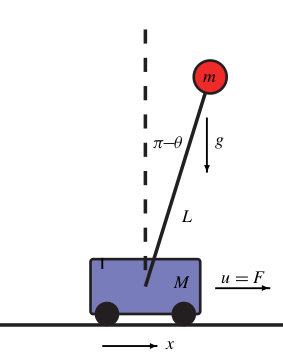
\includegraphics[width = 0.5\columnwidth]{cart-pole.png}
		\caption{Pendule inversé sur un chariot.}
		\label{fig:cart-pole}
	\end{figure}
	Soit un pendule inversé sur un chariot (voir \cref{fig:cart-pole}) dont l'équation dynamique est donné par 
	\begin{align}
		\begin{split}
			\dot{x}&=v\\
			\dot{v}&=\frac{-m^2L^2g\cos(\theta)\sin(\theta)+mL^2(mL\omega^2\sin(\theta)-\delta v)+mL^2u}{mL^2\left(M+m(1-\cos^2(\theta))\right)}\\
			\dot{\theta} &= \omega\\
			\dot{\omega} &= \frac{(m+M)mgL\sin(\theta)-mL\cos(\theta)(mL\omega^2\sin(\theta)-\delta v)-mL\cos(\theta)u}{mL^2\left(M+m(1-\cos^2(\theta))\right)}
		\end{split},
	\end{align}
	où $m$ est la masse du pendule, $M$ est la masse du chariot, $L$ est la longueur du bras, $g$ est l'accélération de la gravité,  et $\delta$ est le coéfficient de frottement sur le chariot.
	\begin{enumerate}
		\item Suivre les mêmes questions du Travail pratique encadré 1, avec $\state_{\rm f}^T = \begin{bmatrix}
			0 & 0 & 0 & 0
		\end{bmatrix}$ et $\out^T = \begin{bmatrix}
		x & \theta
		\end{bmatrix}$.
	\end{enumerate}
\end{tpe}